\section{Editare draft}\label{editare-draft}

Întrucât extragerea informațiilor nu este un proces robust, datele extrase trebuie validate de utilizator. Odată ce imaginile sunt procesate, datele extrase sunt salvate în baza de date, sub categoria \emph{drafts}. În acest moment, bonurile sunt editabile. Figura \ref{fig:draftList} prezintă ecranul unde utilizatorul vede toate drafturile, iar figura \ref{fig:draftScreen} ilustrează ecranul de editare.

\begin{figure}[!ht]
  \centering
  \begin{subfigure}{0.49\textwidth}
    \centering
    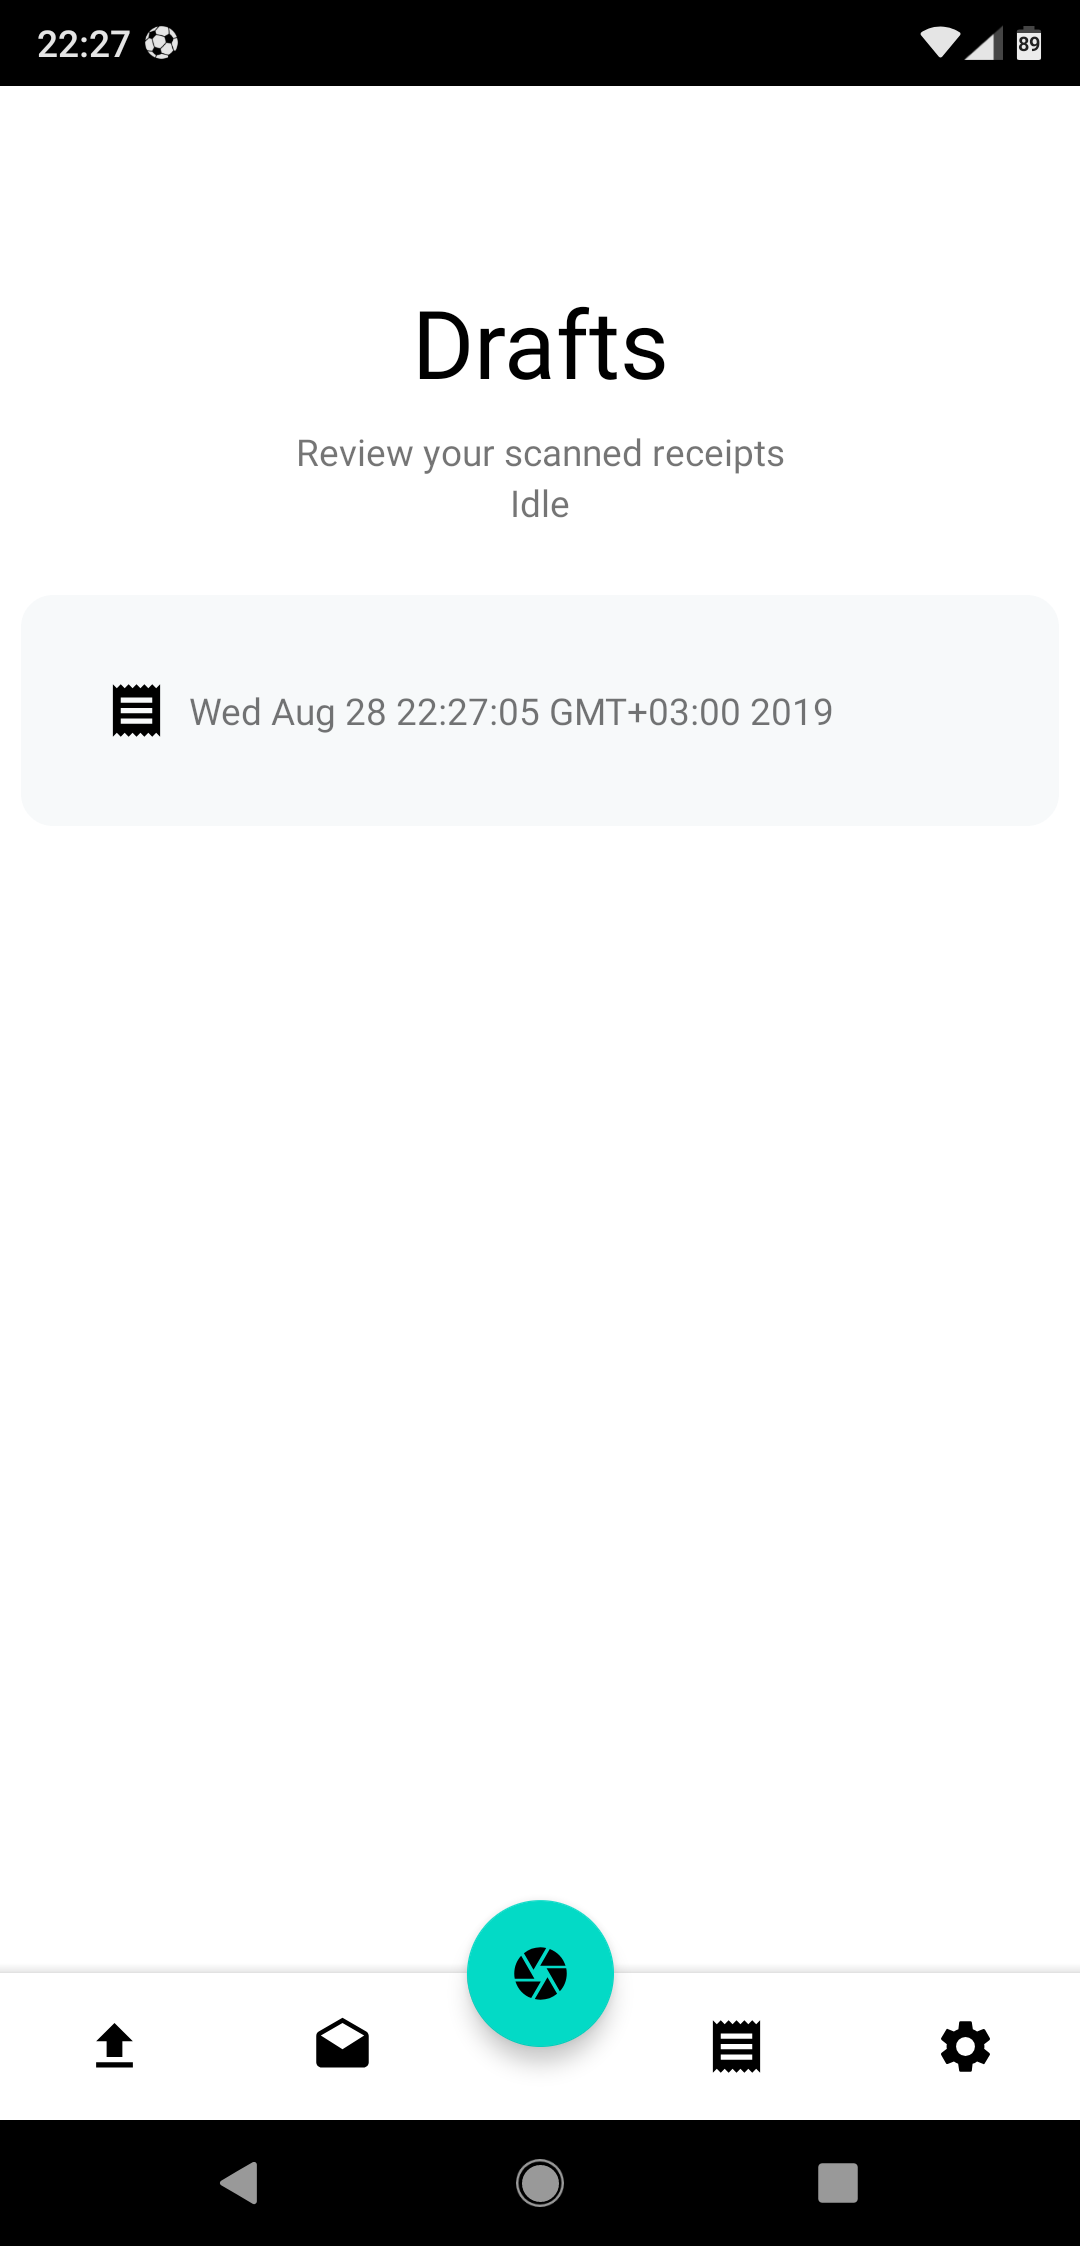
\includegraphics[width=\screenwidth]{DraftsList.png}
    \caption{Ecranul de listare}
    \label{fig:draftList}
  \end{subfigure}
  \begin{subfigure}{0.49\textwidth}
    \centering
    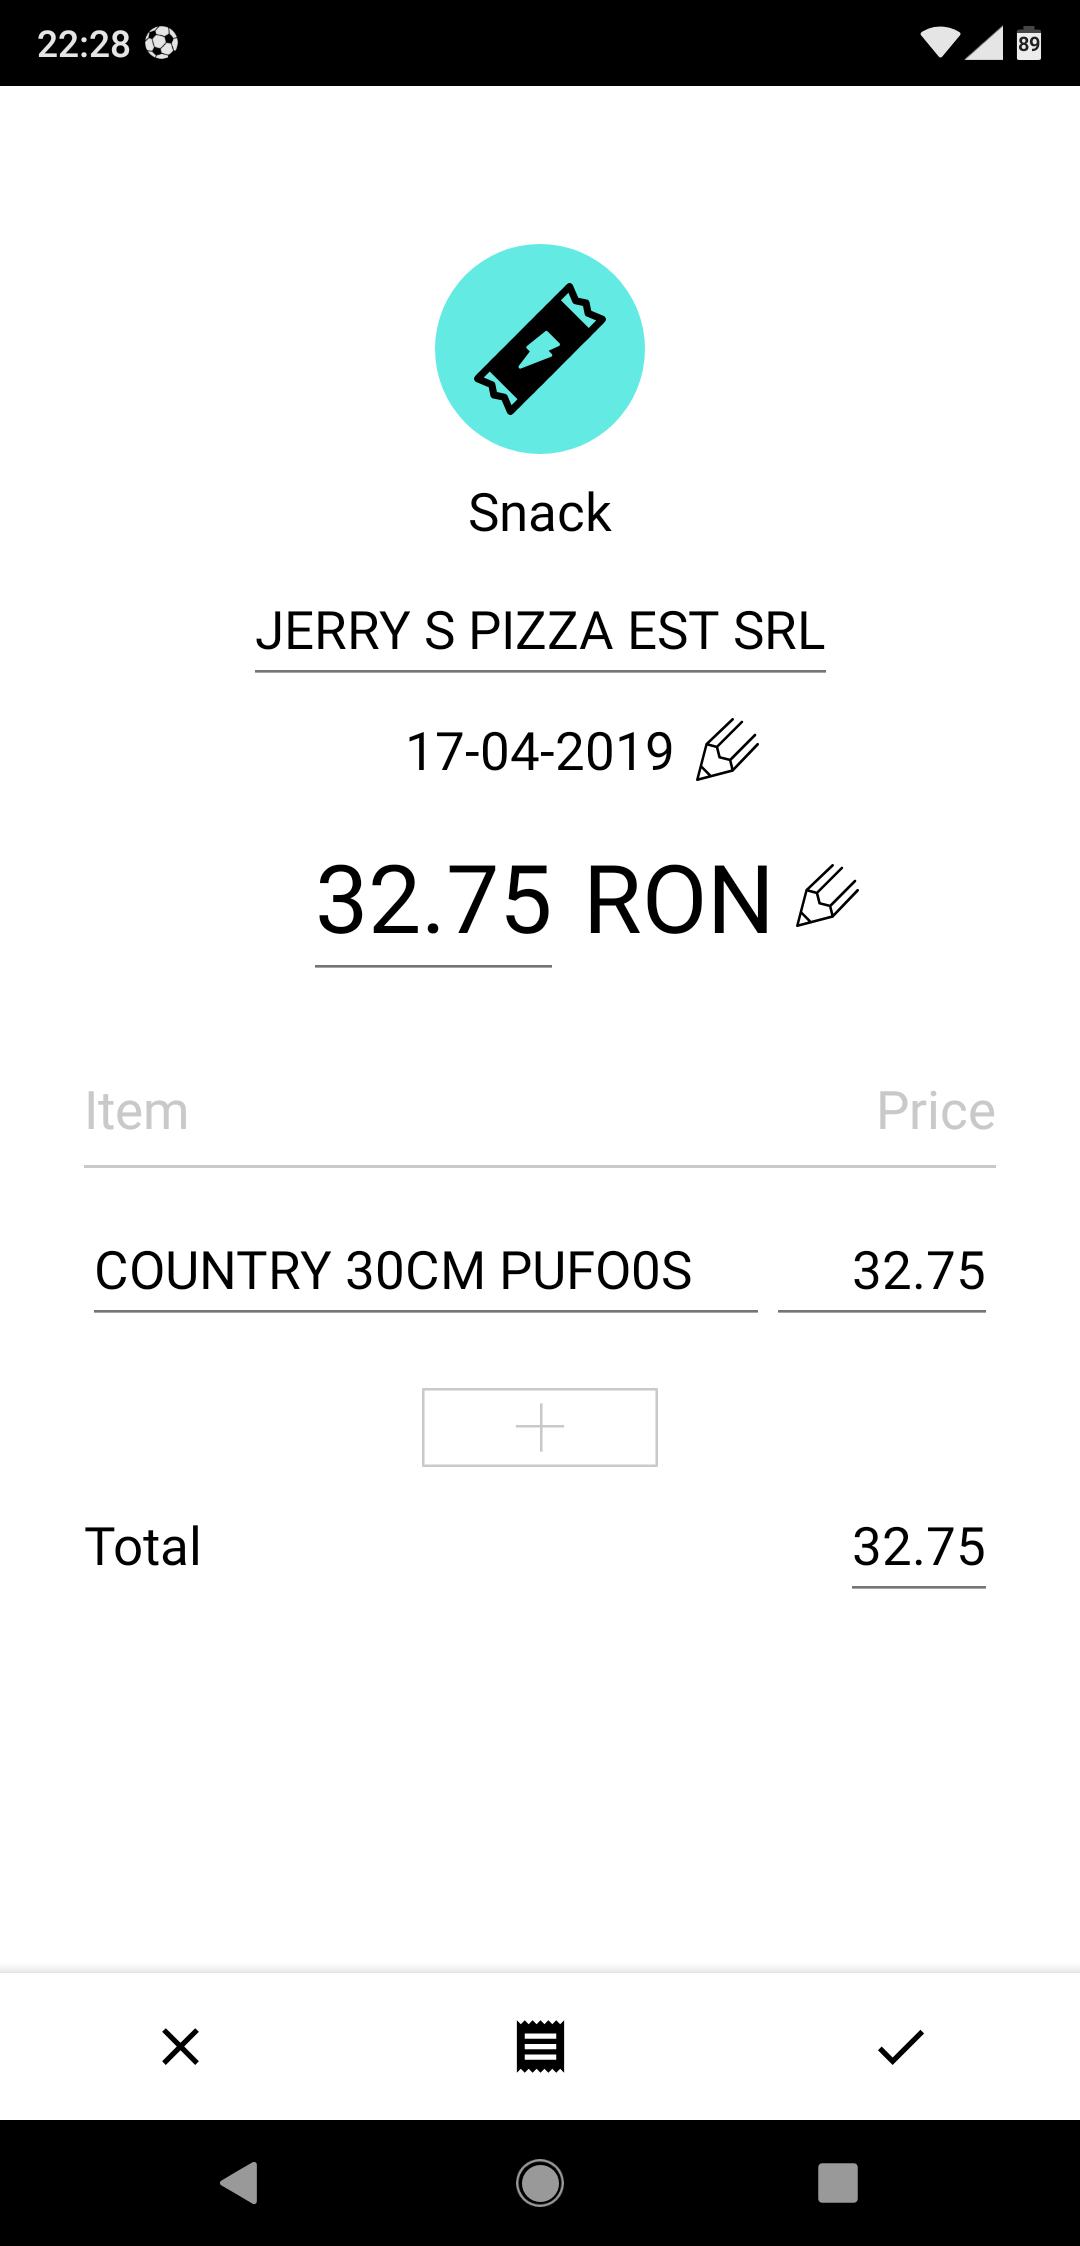
\includegraphics[width=\screenwidth]{DraftScreen.png}
    \caption{Ecranul de editare}
    \label{fig:draftScreen}
  \end{subfigure}
  \caption{Ecranele de gestionare a drafturilor}
  \label{fig:drafts}
\end{figure}

\begin{itemize}
\item
  \textbf{Scop}: Validarea informațiilor extrase din imagine de către utilizator;
\item
  \textbf{Condiție de succes}: Modificările făcute de utilizator se reflectă în baza de date; Bonul este validat și marcat ca final;
\item
  \textbf{Condiții de eșec}: Modificările nu pot fi persistate; Modificările sunt invalide;
\end{itemize}

\subsection*{Mențiuni}

Algoritmul de validare poate fi subiectul unor modificări ulterioare și trebuie să fie ușor de înlocuit.

Validarea considerată la momentul scrierii presupune ca niciun câmp să nu fie null sau fără conținut.

Asupra unui draft, utilizatorul are la dispoziție următoarele opțiuni:
\begin{multicols}{2}
\begin{itemize}
  \item
    modificarea categoriei, prin apăsarea pe ilustrația corespunzătoare;
  \item
    modificarea numelui comerciantului;
  \item
    modificarea datei, prin folosirea unui \emph{date picker};
  \item
    modificarea prețului total și a monedei;
  \item
    modificarea numelui sau prețului unui produs;
  \item
    ștergerea unui produs, prin gestul de \emph{swipe};
  \item
    adăugarea unui produs, prin apăsarea butonului de adăugare;
  \item
    ștergerea sau validarea \emph{draft-ului} și vizualizarea imaginii aferente prin butoanele din bara de opțiuni;
\end{itemize}
\end{multicols}

\subsection*{Principalul scenariu}


% \begin{minsipage}[t]{0.55\textwidth}

\begin{enumerate}
\item
  Utilizatorul accesează un bon;
\item
  Utilizatorul modifică câmpurile dorite;
\item
  Utilizatorul cere validarea bonului; Validarea se efectuează cu succes;
\item
  Bonul este scos din lista \emph{drafts} și pus în lista bonurilor validate;
\end{enumerate}

% \end{minipage} \vspace{0.01\textwidth}
% \begin{minipage}[t]{0.44\textwidth}

\subsection*{Variații}

\begin{itemize}
\item
  Utilizatorul poate modifica valori, dar fără a valida bonul;
\item
  Utilizatorul poate valida bonul, ceea ce îl scoate din lista de \emph{drafts} și îl pune în lista de bonuri valide;
\item
  Accesarea unui bon se face fie prin alegerea acestuia din listă, fie în urma scanării unei imagini; (Înțelegerea imaginilor)
\end{itemize}
% \end{minipage}
  
\subsection*{Extensii}

\begin{itemize}
\item
  Utilizatorul poate vedea imaginea capturată, cu și fără elementele OCR;
\item
  Utilizatorul poate vedea toate bonurile din lista \emph{drafts} și poate naviga către unul din ele;
\end{itemize}


